\documentclass[aspectratio=169,10pt]{beamer}
\usepackage{common/pdmtheme}
\graphicspath{{figures/}}
\title[Alif E7 node]{Alif Ensemble E7}
\subtitle{What an NPU microcontroller actually buys --- measured, not assumed}
\author{Predictive Maintenance Platform}
\date{13 October 2026}
\begin{document}

\begin{frame}[plain]
  \vspace{5mm}
  {\LARGE\bfseries Alif Ensemble E7}\\[2mm]
  {\large\color{pdmink2} What an NPU microcontroller actually buys}\par
  \vspace{5mm}\noindent{\color{pdmrule}\rule{\linewidth}{0.4pt}}\par
  \vspace{3mm}
  \begin{columns}[T]
    \begin{column}{0.46\textwidth}
      \scriptsize
      \kv{Cores}{M55 HE 160 MHz + M55 HP 400 MHz}\\[1mm]
      \kv{NPU}{2$\times$ Ethos-U55, 128 and 256 MAC}\\[1mm]
      \kv{SRAM}{5.5 MB on-chip}\\[1mm]
      \kv{Helium}{MVE --- halves the FFT}\\[1mm]
      \kv{Compute share}{\textbf{1.2 \% of the energy cycle}}\\[1mm]
      \kv{Battery life}{1.50 y --- \emph{slightly worse} than the STM32U5}
    \end{column}
    \begin{column}{0.46\textwidth}
      \scriptsize\color{pdmink2}
      \textbf{Never flashed.} And the kit's reason for existing --- the waveform
      model on the NPU --- is \textbf{not written}. Writing it needs a 1D CNN
      trained on measured data, which no model in this repository has yet been.
      \\[2mm]
      A stub returning a plausible probability would make the kit look complete
      and would be the most misleading artefact here.
    \end{column}
  \end{columns}
  \srcnote{Branch \texttt{hw/alif-e7-ethos-u55}.}
\end{frame}

% -------------------------------------------------------------- the answer ---
\begin{frame}{On the baseline pipeline, the NPU does nothing}
  \centering
  \scriptsize
  \begin{tabular}{@{}lrr@{}}
    \toprule
    & \textbf{Latency} & \textbf{Share of the energy cycle} \\
    \midrule
    63-float detector, plain C       & $\sim$23 $\mu$s & 0.011 \% \\
    \quad CMSIS-NN on the M55        & $\sim$8 $\mu$s  & --- \\
    \quad \textbf{Ethos-U55}         & $\sim$2 $\mu$s  & --- \\
    Whole DSP pipeline (Helium)      & 2.4 ms          & 1.2 \% \\
    \textcolor{pdmcrit}{\textbf{Acquisition window}} & \textcolor{pdmcrit}{\textbf{307 ms}} & \textcolor{pdmcrit}{\textbf{66.9 \%}} \\
    \bottomrule
  \end{tabular}
  \\[3mm]
  \begin{columns}[T]
    \begin{column}{0.48\textwidth}
      \scriptsize
      An NPU that takes inference from 23 $\mu$s to 2 $\mu$s is optimising
      \textbf{0.010 \%} of the budget. Helium, which halves the FFT, optimises
      1.2 \%.
      \\[1mm]
      \color{pdmink2}\footnotesize
      These were 0.0005 \% and 0.5 \% until the energy model's acquisition
      window was corrected from a flat 1000 ms to this firmware's 307 ms. The
      NPU figure moved by 20$\times$ and the conclusion did not --- which says
      it was never resting on the number.
      \\[1.5mm]
      A node on this part has materially the same battery life as one on a
      90 EUR STM32U5 --- in fact \emph{slightly worse}, because the sleep
      current is a little higher.
    \end{column}
    \begin{column}{0.48\textwidth}
      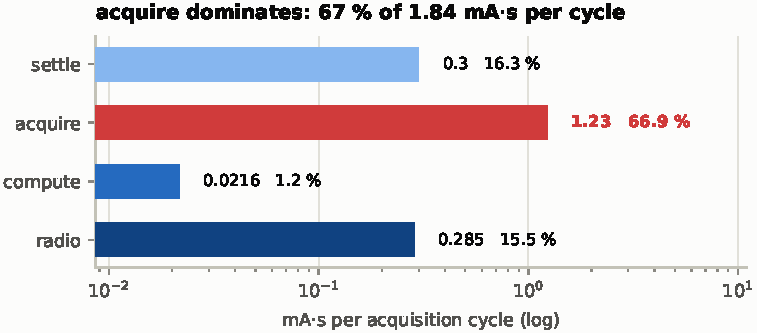
\includegraphics[width=\linewidth]{kit_alif_e7_energy.pdf}
    \end{column}
  \end{columns}
  \takeaway{Every ``AI microcontroller'' evaluation should start with this table.
    On a low-duty sensor the dominant term is the sensor, not the maths.}
\end{frame}

% --------------------------------------------------------------- the point ---
\begin{frame}{What it does buy: a model that does not otherwise fit}
  \centering
  \begin{tikzpicture}[node distance=4mm and 8mm]
    \node[pdmblk, minimum width=24mm] (acq) {acquisition\\\tiny 8192 @ 26.667 kHz};
    \node[pdmblk3, minimum width=36mm, above right=2mm and 12mm of acq] (feat)
      {63-float detector, HE core, 2 $\mu$s\\\tiny \textbf{PRIMARY} --- comparable across all 8 kits};
    \node[pdmblk2, minimum width=36mm, below right=2mm and 12mm of acq] (cnn)
      {2048-sample 1D CNN, HP + NPU, 0.25 ms\\\tiny \textbf{EXPERIMENT} --- off by default};
    \draw[pdmarrow] (acq.east) -- (feat.west);
    \draw[pdmarrowalt] (acq.east) -- (cnn.west);
  \end{tikzpicture}
  \\[3mm]
  \begin{columns}[T]
    \begin{column}{0.48\textwidth}
      \scriptsize
      At $\sim$20 GMAC/s the small Ethos-U55 runs a 2--5 MMAC 1D CNN over the
      raw waveform in \textbf{0.25 ms}. The same model is 100--250 ms on the HE
      core alone and $\sim$600 ms on the nRF9160's 64 MHz M33 --- longer than
      the acquisition it would be analysing.
      \\[1.5mm]
      That architecture is what the 2025--2026 literature actually uses:
      end-to-end 1D CNN on raw vibration, dual-domain multi-scale CNN at
      $-4$ dB SNR, lightweight on-device transformers. \emph{None of them run on
      any other kit here.}
    \end{column}
    \begin{column}{0.48\textwidth}
      \scriptsize
      \textbf{Why the experiment is off by default}
      \\[1mm]
      $\bullet$ \textbf{Comparability.} Eight kits exist to be compared; a
      different default produces frames that cannot sit beside the others.\\[1mm]
      $\bullet$ \textbf{Energy.} Running it every cycle costs more than the
      whole rest of the cycle --- and 99.99 \% of acquisitions are on healthy
      machines.\\[1mm]
      $\bullet$ \textbf{Epistemics.} The result is reported \emph{alongside} the
      feature frame. The interesting output is the \textbf{disagreement set};
      replacing the comparable path destroys the only evidence that would settle
      which model is right.
    \end{column}
  \end{columns}
  \takeaway{The NPU changes which hypothesis the node can test --- not how fast
    it tests the current one.}
\end{frame}

% --------------------------------------------------------------- gating ------
\begin{frame}{Power domains matter more than TOPS; and one flag costs 2\texttimes}
  \begin{columns}[T]
    \begin{column}{0.48\textwidth}
      \small\textbf{The HP core must be \emph{absent}, not idle}
      \\[1.5mm]
      \scriptsize
      \begin{tabular}{@{}lrr@{}}
        \toprule
        & \textbf{Current} & \textbf{Role} \\
        \midrule
        M55 HE, 160 MHz & 4.5 mA  & the whole normal cycle \\
        M55 HP, 400 MHz & 22 mA   & \textbf{powered off} \\
        \bottomrule
      \end{tabular}
      \\[2mm]
      22 mA left \emph{idle} between hourly acquisitions costs 79 mA$\cdot$s per
      hour --- \textbf{17$\times$ the entire rest of the cycle}.
      \\[1.5mm]
      So the real argument for a heterogeneous SoC in a battery application is
      about \emph{gating}, not throughput. A part whose big core cannot be fully
      powered down is worse here than a small one, whatever its TOPS figure.
    \end{column}
    \begin{column}{0.48\textwidth}
      \small\textbf{\texttt{-mfpu=auto}}
      \\[1.5mm]
      \scriptsize
      On a Cortex-M55 this flag is what enables MVE. Without it the compiler
      emits scalar code, CMSIS-DSP silently falls back to its generic paths, and
      the FFT takes twice as long.
      \\[1.5mm]
      \textbf{It produces identical numbers.} Golden vectors match. Edge/cloud
      feature agreement matches. Quantisation round-trip matches. \emph{Every
      test in this repository passes either way.}
      \\[1.5mm]
      A 2$\times$ regression invisible to the whole test suite is exactly the
      kind of defect that ships. The only detection is a PMU cycle count on
      hardware --- which is why it is on the checklist and why the flag carries
      a comment rather than just being set.
      \\[1.5mm]
      Same hazard on the NPU: Vela's operator fallbacks are silent, and one
      unsupported operator runs on the CPU at 1/100th the speed with the same
      answer.
    \end{column}
  \end{columns}
\end{frame}

\end{document}
